\section{Experimental Evaluation}\label{sec:eval}

\begin{figure}[t]
  \begin{adjustwidth}{-0.13\textwidth}{-0.13\textwidth}
  	\centering
    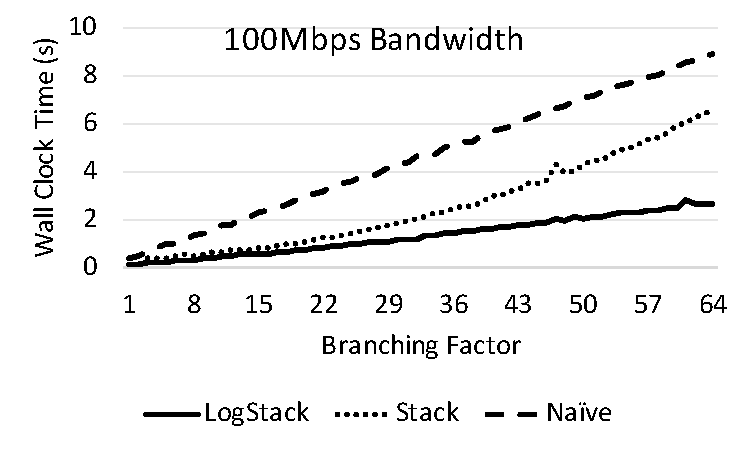
\includegraphics[width=0.4\textwidth]{fig/100mbps}
    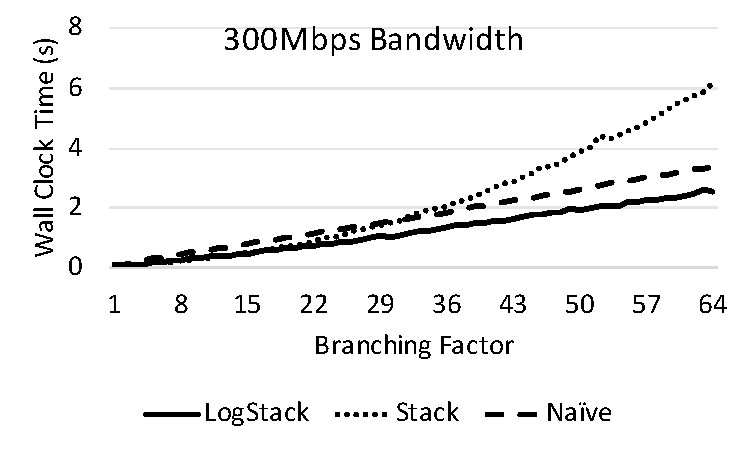
\includegraphics[width=0.4\textwidth]{fig/300mbps}
    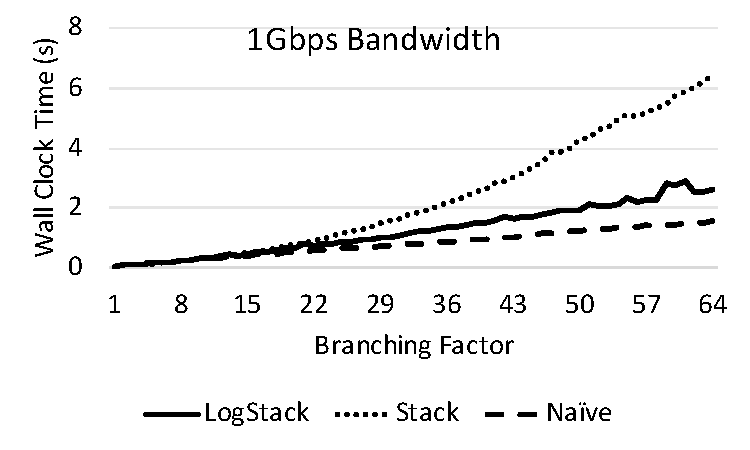
\includegraphics[width=0.4\textwidth]{fig/1gbps}
  	\\
    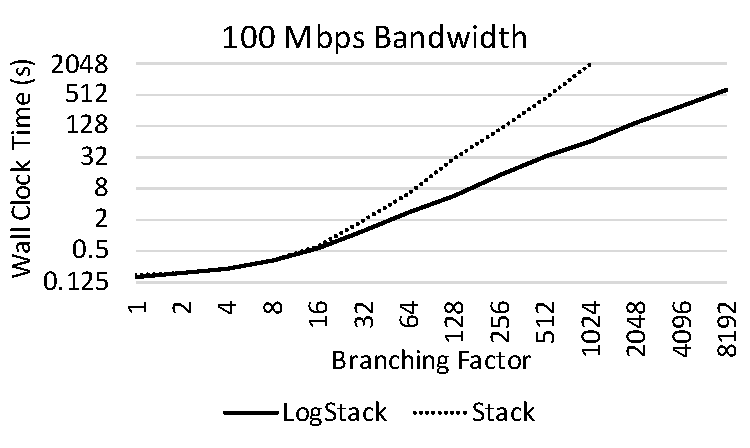
\includegraphics[width=0.4\textwidth]{fig/highbranching}
    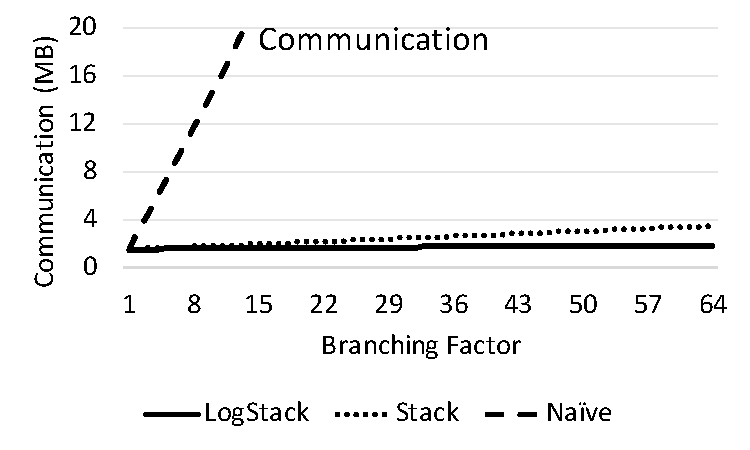
\includegraphics[width=0.4\textwidth]{fig/comm}
    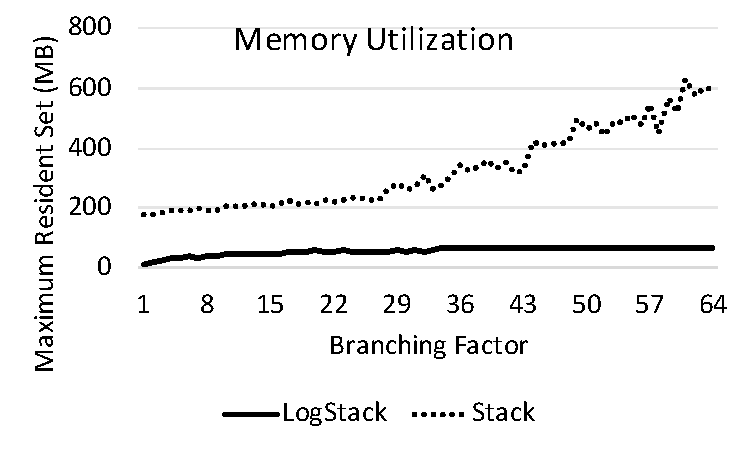
\includegraphics[width=0.4\textwidth]{fig/memutil}
  \end{adjustwidth}
  \caption{%
  }\label{fig:plots}
\end{figure}

We implemented \ourschemelong and extensively experimented with it and with implementations of basic half-gates~\cite{EC:ZahRosEva15} and the \stack SGC of~\HK.
We report on our experimental evaluation, and compare in detail to  basic half-gates~\cite{EC:ZahRosEva15} and to~\HK.  Charts of \Cref{fig:plots} present and summarize the results of our experiments.

We consider  the following metrics: end-to-end wall-clock time performance, bandwidth consumption, and memory utilization of 2PC implemented with each of the three schemes and executed with varying number of branches.  All branches implement the SHA-256, which has XX AND gates and XX XOR gates.  A GC for each branch has size XX MB.  As discussed in~\Cref{sec:instantiation}, we ensure that our implentation does not take shortcuts due to branches implementing the same function.

\paragraph{Bandwidth}  is the easiest to observe, analyze and discuss.  The communication chart of~\Cref{fig:plots} plots the communication in MB for number of branches from 1 to 64.  As expected, both \stack and \ourschemelong communication remains almost constant, while half-gates grows linearly and immediately dominates.  \ourschemelong is slightly leaner than \stack because XXX.

\paragraph{Memory Utilization} is measured for number of branches from 1 to 64.  We compare our scheme to \stack (half-gates memory utilization will be constant in the number of branches, since state associated with processed branches can be discarded).  While \stack uses a modest amount of RAM in our experiments, our experiments are on relatively small circuits.  For larger branch sizes and more branches, its memory consumption may become a bottleneck.  In contrast, our memory utilization scales well both with increased branch size and the number of branches.  For example, we executed our implementation on a circuit with $8192$
SHA-256 branches, a circuit that altogether holds $> 385$M AND-gates.
Our peak memory usage was at around $100$MB, while \HK would require more
than $12$GB of space to run this experiment.

\paragraph{Total wall-clock time} is complete metric, and as such, it conveys a bigger, less nuanced picture.  We plot three charts for 1-64 branches (100, 300 and 1000 Mbps) comparing each of the three approaches.  We explore more extreme conditionals of up to 8192 branches in the 100Mbps setting.

In the 1Gbps network setting, as expected, na\"ive half-gates leads.  As discussed in~\Cref{sec:whentouse}, two cores (our laptop) indeed cannot keep up with the available network capacity.  However, doubling number of course already puts us ahead of na\"ive, and any further computation boost correspondingly further improves \ourschemelong vs na\"ive.  We are about $3\times$ faster than \stack.

In the 300Mbps network setting we are already always better than na\"ive.  Because we range over the same number of branches (up to $64$) we are the same factor $\approx 3\times$ faster than \stack.

The more typical $100$Mbps setting shows off advantage of stacking.  Both \stack and \ourschemelong handily beat na\"ive.

Finally, we experiment with very large number of branches.  \ourschemelong scales well and we garbled up to $8192$ circuits as it was sufficient to demonstrate a trend.  \ourschemelong would run on an arbitrary number of circuits.  In contrast, \stack exhibited a much more limited scaling capacity.  We ran up to $512$ branches with \stack, enough to demonstrate a trend, and after which our experiments started to consume too much time.   \ourschemelong garbled a $512$-branch conditional in $\approx 32s$, while \stack took $\approx 2053s$,  $64\times$ slower than \ourschemelong.


